\chapter{Experiments and Evaluation Metrics}

In this chapter we will go over the various experiments and metrics used to evaluate the performance of our methods. This information is subsequently divided into three sections.

In the first section we will show the metrics used to describe the performance of the pose estimation network.

In the second section we will then show how we evaluated the performance of our semantic meaning extraction strategy.

Finally, in the third section we will discuss the experimental setup we used to test the performance of our complete model in a real-life robotics application.

\section{Evaluation Metrics for Pose Esitmation and Object Detection}

Most pose estimation and object detection methods share a common set of metrics on which their performance is evaluated. These are namely Average Precision for object detection strategies, and Average Distance and ADD for pose estimation strategies. In this section we will describe each metric, its meaning and how it is computed.

\subsection{Average Precision}

The performance of object detectors and 2D bounding box regressors is usually evaluated using median Average Precision (mAP), which is a descriptor of the reliability of a method's predictions. It exploits the intersection over union (IoU), computed as:

\begin{equation*}
    \text{IoU} = \frac{B_{GT} \cap B_{P}}{B_{GT} \cup B_{P}}
    \label{eq:IoU}
\end{equation*}

where $B_{GT}$ is the area of the ground truth bounding box and $B_{P}$ is the area of the network's predicion. A prediction is considered true if its IoU is greater than a threshold; based on this, we can generate the model's confusion matrix, as described in table \ref{confusionmatrix}.

\begin{table}[ht]
    \begin{center}
        \begin{tabular}{c||c|c}
            \space & Actual Positives & Actual Negatives\\
            \hline\hline
            Predicted Positives & True Positives (TP)& False Positives (FP)\\
            \hline
            Predicted Negatives & False Negatives (FN)& True Negatives (TN)\\
        \end{tabular}
        \caption{Generation of the confusion matrix.}
        \label{confusionmatrix}
    \end{center}
\end{table}

This matrix is the basis for the definition of the precision and recall metrics. Precision is an indicator of how well the model avoids false positives, while recall is an indicator of how well a model avoids false negatives. They are computed as follows:

\begin{align*}
    \text{Precision (P)} &= \frac{\text{TP}}{\text{TP} + \text{FP}}\\
    \text{Recall (R)} &= \frac{\text{TP}}{\text{TP} + \text{FN}}
\end{align*}

Precision and recall both depend on the value of the threshold: smaller thresholds will result in a more restrictive model, thus less false positives and more false negatives, high precision and low recall, while high thresholds will result in the opposite: more false positives, less false negatives, low precision and high recall.

It is common practice to plot the precision as a function of the recall in what is called a precision-recall curve, $P = f(R)$. Each point in the curve represents a value of the threshold, corresponding to its own confusion matrix and subsequent metrics. An example plot is shown in figure \ref{example_pr}.

\begin{figure}[ht]
    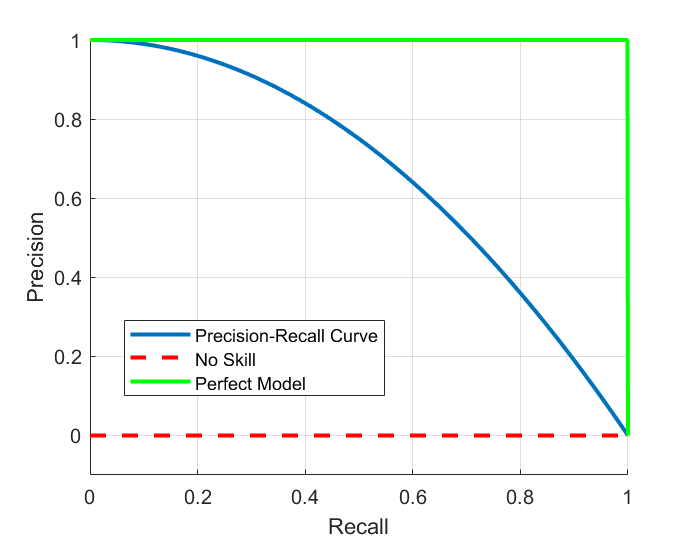
\includegraphics[width=0.6\textwidth]{example_pr_curve.png}
    \caption{Example of precision recall curves. The red line indicates a model with no skill at a task, thus zero precision; the blue line a model with some skill; the red line is the ideal behavior with maximum precision and recall at all times.}
    \label{example_pr}
\end{figure}

At this point we can describe the Average Precision (AP) as the mean value of the precision, corresponding to the area under the precision-recall curve:

\begin{equation*}
    \text{AP} = \int_{0}^{1} f(R)dR
\end{equation*}

The median Average Precision is then obtained as the average AP over all object classes:

\begin{equation*}
    \text{mAP} = \frac{1}{n} \sum_{i=1}^{n} \text{AP}_{i}
\end{equation*}

Therefore it is a real value between 0 and 1, with 0 representing the model with no skill, and 1 representing the ideal behavior.

\subsection{Average Distance and ADD}

Evaluation of pose estimation methods is almost exclusively done using the ADD metric, and by extension the Average Distance (AD). While the first is an indicator of the percentage of correct estimations, similar in a sense to mAP, the second is instead unique to pose estimation.

Given $n$ points belonging to the 3D model $M$ of an object, the AD represents the average of the distance between these points transformed according to the ground truth ($\text{R}, \text{t}$) and according to the prediction ($\hat{\text{R}}, \hat{\text{t}}$):

\begin{equation*}
    \text{AD} = \frac{1}{n} \sum_{x \in M} ||(\text{R}x + \text{t}) - 
    (\hat{\text{R}}x + \hat{\text{t}})||_2
\end{equation*}

The ADD is then given by the percentage of correct poses given by the model. A pose is correct if its AD metric is less than 10\% of the 3D model's diameter.

This metric has been in use since before the introduction of neural networks to pose estimation, but it runs into serious issues when dealing with objects that have rotational symmetry. The reason for this is that these objects may present no visual differences with different rotations. For example, one image of the M6x30 screw we use for inferencing could correspond to six different poses, each varying 60\degree from the previous one. This means that the model will eventually stabilize at a value that minimizes the average error, which is ususally large.

To combat this issue, we use the Symmetric Average Distance (AD-S)\cite{PoseCNN} metric, defined as the average minimum distance between points in the predicted pose and the ground truth:

\begin{equation*}
    \text{AD-S} = \frac{1}{n} \sum_{x_1 \in M} \min_{x_2 \in M} ||(\text{R}x_2 + \text{t}) - 
    (\hat{\text{R}}x_1 + \hat{\text{t}})||_2
\end{equation*}

This is very similar to the loss used in the ICP algorithm, as it only considers the distance from each point to its closest correspodent in the ground truth. Analogously to ADD, we then implement ADD-S as the percentage of correct poses.

Finally, we can introduce the Mixed Average Distance, which is defined as:

\begin{equation*}
    \text{ADD(-S)} = 
    \begin{cases}
        \text{ADD-S} & \text{if the object is symmetric,}\\
        \text{ADD} & \text{otherwise.}
    \end{cases}
\end{equation*}

We would like our model to have the highest possible ADD, however in an industrial environment it is important to also evaluate the AD. This is because for larger objects the ADD will tolerate greater estimation errors, as it is based on the diameter of the objects; these errors however may not be compatible with the precision required for a determined task.

\section{Semantics Evaluation Methodology}
\label{semantics_method_section}

To evaluate our semantic meaning extraction method, we must compare ground truth values for the semantic state of each scene, associated with its own image, with the outputs of our method.

Our strategy therefore is to save the semantic state for each image during dataset generation. We then run the trained model on a subset of these images, coinciding with the test set, to obtain predictions, and then run our semantic meaning extraction method on the predictions.

However, an issue arises from the application of this method. Due to the symmetry of the boards, it is impossible to determine visually which slot is which. For example in figure \ref{sym_eval}, the ground truth is that there is a button in the first slot, however the model outputs the button in the second slot. Visually, both of these interpretations are correct, since the board is symmetrical, however directly comparing the output with the ground truth results in two "false" values.

\begin{figure}[ht]
    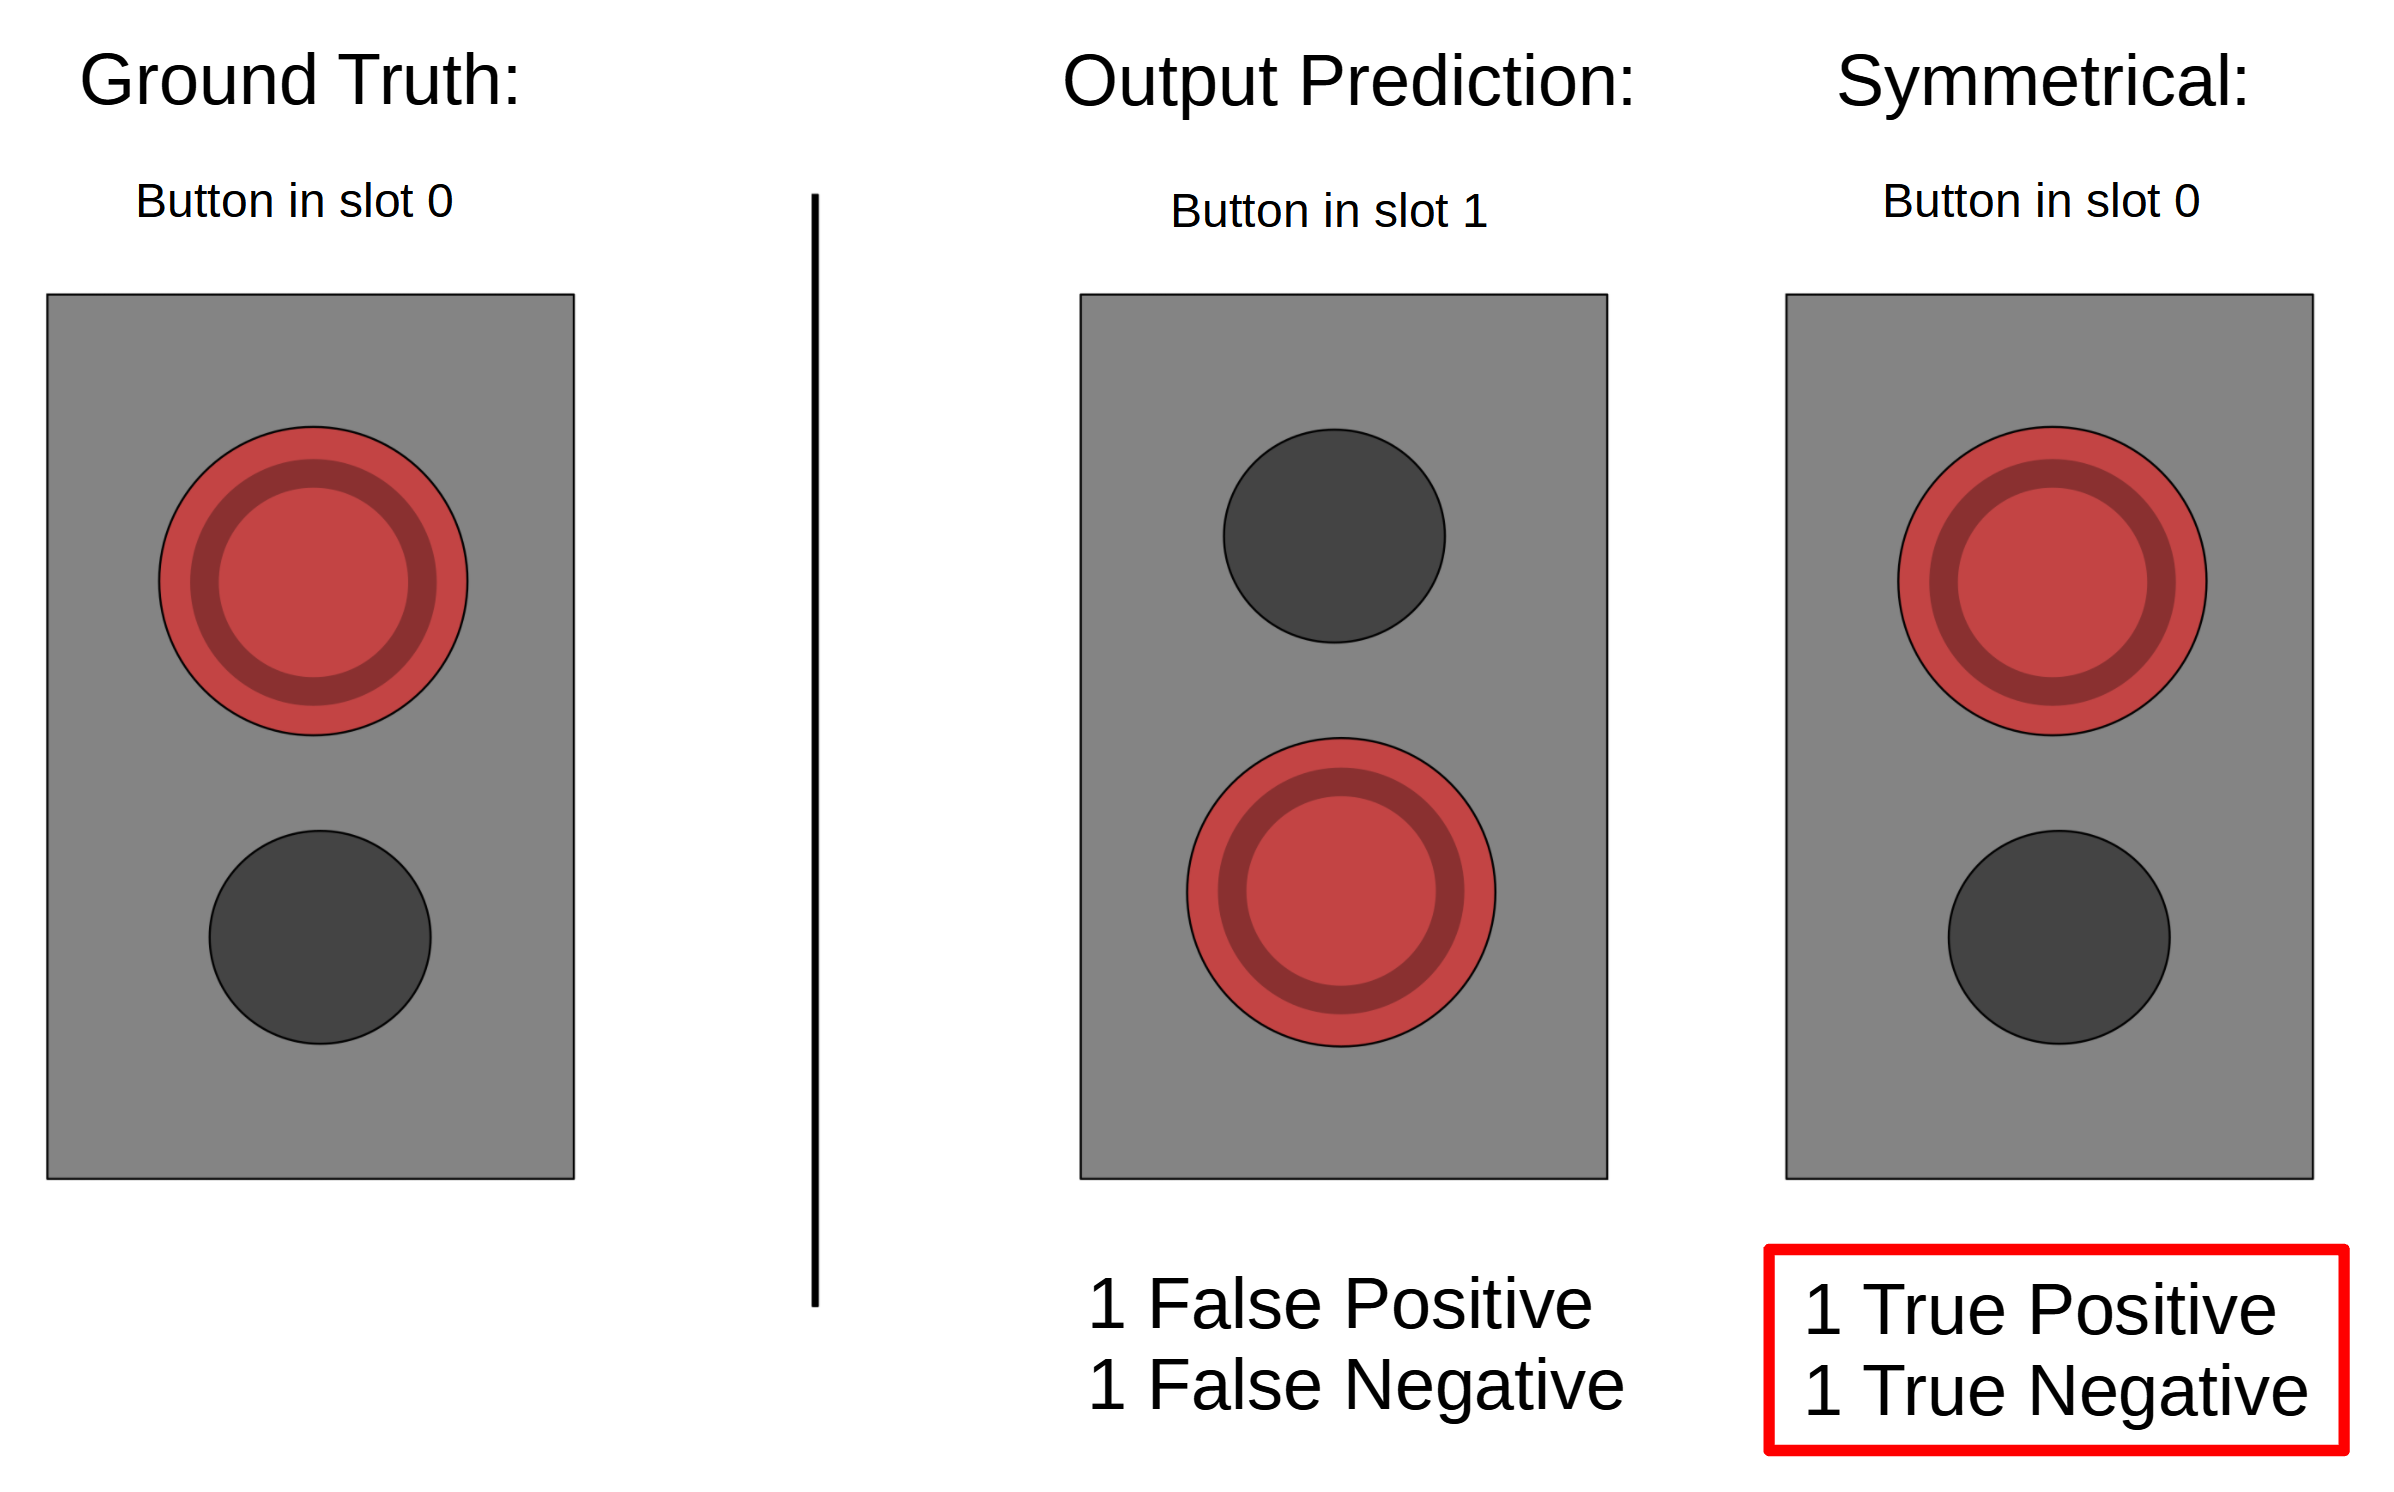
\includegraphics[width=0.8\textwidth]{sym_evaluation.png}
    \caption{Selection between the model's output and its symmetrical when evaluating the semantic state of a scene.}
    \label{sym_eval}
\end{figure}

To combat this issue, we consider both the model's output, and its symmetrical condition, and take the results from the version with the greatest number of true values when compared with the ground truth. Therefore we compare both the model output and its symmetrical: since the symmetrical results in two "true" values, the final output of the comparison is two "true" values: a true negative and a true positive.

Once this issue has been resolved, we can build for each given threshold a confusion matrix as described in the previous section, and compute a precision-recall curve.

To select the optimal threshold, we consider the F1 score, which is a balanced function of precision and recall, computed as:

\begin{equation*}
    \text{F1} = 2\times\frac{\text{Precision}\times\text{Recall}}{\text{Precision}+\text{Recall}}
\end{equation*}

We consider the optimal threshold to be the one that maximises this value.

\begin{figure}[ht]
    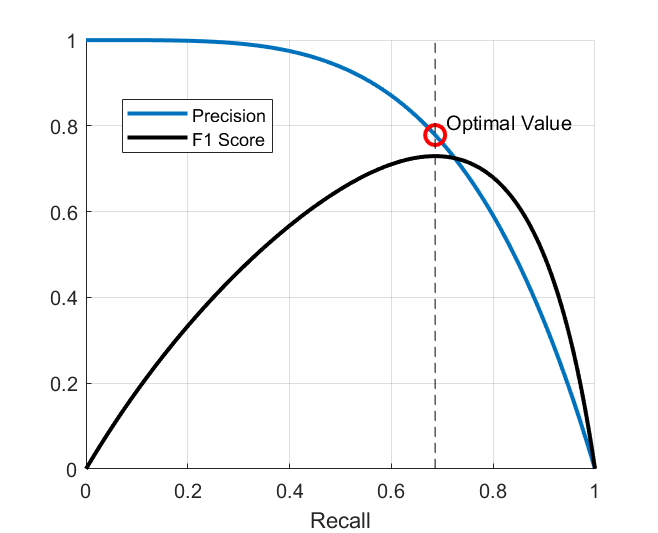
\includegraphics[width=0.5\textwidth]{best_f1_example.png}
    \caption{Example of selecting the optimal threshold using the maximum of the F1 curve.}
\end{figure}

\section{Real-Life Experimental Setup}

To test the effectiveness of our vision and semantics model, we will be implementing it in a real life situation where we have to complete a simple assembly task. We will be using a Doosan A0509s robotic manipulator equipped with a pneumatic gripper, and an Azure Kinect camera. We will be re-utilizing previously developed code for this system that generates behaviour trees \cite{behavior_tree} to drive the robot based on previous demostrations of actions and their effects on the scene.

First, we must describe each scene using a list of predicates. These predicates are first-order logic functions that can be either true or false, and must be evaluated each time we obtain new information on the scene. A list of these predicates and their descriptions is supplied in figure \ref{predicateslist}.

\begin{table}[ht]
    \begin{center}
        \begin{tabular}{cc}
            Predicate & Description \\
            \hline \hline
            IsGripperEmpty(gripper) & True when no objects are in the gripper. \\
            \hline
            IsGrapsed(Button, Gripper) & True when the button is grasped by the gripper. \\
            \hline
            IsButtonInSlot(Button, Slot) & True when the button is inserted in the slot. \\
            \hline
            IsSlotEmpty(Slot) & True when no buttons are in the slot.\\
        \end{tabular}
        \caption{List of predicates used to describe scenes in our application, with descriptions.}
        \label{predicateslist}
    \end{center}
\end{table}

Once these predicates are available and can be evaluated, we can "teach" the robot to perform actions through kinesthetic demostrations. During these demostrations, the robot, moved by a human operator, will modify the environment and thus change the state of the scene. Since this state can be described using a list of predicates, we can save the differences between the inital state and the final state to understand the pre-requisites and consequences of each action in predicate form. We then use Planning Domain Definition Language (PDDL) \cite{pddl} to define each action and unite these definitions into a domain description. For example, if we take our task of picking up a button and inserting it into a slot, the states would be as described in figure \ref{predicatesevolutions}.

\begin{figure}[ht]
    \subfloat[Initial State]{
        \begin{tabular}{c}
            Predicates: \\
            \hline
            IsSlotEmpty(slot) \\
            IsGripperEmpty(gripper) \\
            ... \\
        \end{tabular}
    }

    \subfloat[Intermediate State]{
        \begin{tabular}{c}
            Predicates: \\
            \hline
            IsSlotEmpty(slot) \\
            IsGrasped(button, gripper) \\
            ...\\
        \end{tabular}
    }

    \subfloat[Final State]{
        \begin{tabular}{c}
            Predicates: \\
            \hline
            IsButtonInSlot(button, slot) \\
            IsGripperEmpty(gripper) \\
            ...\
        \end{tabular}
    }

    \caption{Evolution of the state, expressed as a list of predicates, during the pick-up and insertion of a button into a slot.}
    \label{predicatesevolutions}
\end{figure}

The domain for this task would then contain a list of the possible predicates, and two actions: the evolution from the initial state to the intermediate state (picking up the button) and the evolution from the intermediate state to the final state (inserting it into the slot), shown in figure \ref{pddlactions}.

\begin{figure}
    \subfloat[action_0 (Picking up a button)]{
        \begin{tabular}{c|c|c}
            Parameters & Preconditions & Effects \\
            \hline
            gripper & IsGripperEmpty(gripper) & !IsGripperEmpty(gripper) \\
            button & \space & IsGrasped(button) \\
        \end{tabular}
    }
    \subfloat[action_1 (Inserting a button into a slot)]{
        \begin{tabular}{c|c|c}
            Parameters & Preconditions & Effects \\
            \hline
            button & IsGrasped(button) & !IsGrasped(button) \\
            slot & IsSlotEmpty(slot) & !IsSlotEmpty(slot) \\
            gripper & \space & IsGripperEmpty(gripper) \\
            \space & \space & IsButtonInSlot(button, slot) \\
        \end{tabular}
    }

    \caption{Actions with their parameters, preconditions and effects as saved by PDDL for our task.}
    \label{pddlactions}
\end{figure}

We then define an init and goal for our planner, which are the state we are starting from and the final state we want to achieve, compact both of these into the "problem definition". Inputting the definition and the domain into a PDDL planner then gives us the set of actions we need to perform, (in this case action_0 and the action_1), which we can use to then build our behaviour tree.

The main modification applied to the previous code in this approach, apart from changing the predicates to suit our needs, is the shift from a continuously evaluated model to a discretely evaluated model. The reason for this change is the susceptibility of the vision model to false positives for previously unidentified objects. More information on this can be found in section \ref{false_positives_issue}, but essentially in this manner we ensure that the state is evaluated only when the gripper and eventual human operator are outside of the camera's field of view.

